\section{Results}

\subsection{Single-shot model performance}
\label{subsection:single-shot}

Figure \ref{fig:fig_3_singleshot} clearly shows that the tested models have performed differently on different datasets assessed in this study. Namely, for the datasets where the scores were obtained with DOCK (D4 and AmpC), recall scores tend to be higher than for those obtained with ICM.

Also, the increase in the training dataset size does not lead to significant improvements in the models performance, in line with previously observed results \cite{Yang2021_shoichet_active_learning}. Despite that, "heavyweight" models such as RandomForestRegressor, seem to benefit by that more, compared to more "lightweight" linear models, which seem to saturate at train size around $160\ 000$ \ref{fig:fig_3_singleshot}.

\begin{figure}[ht]
\centering
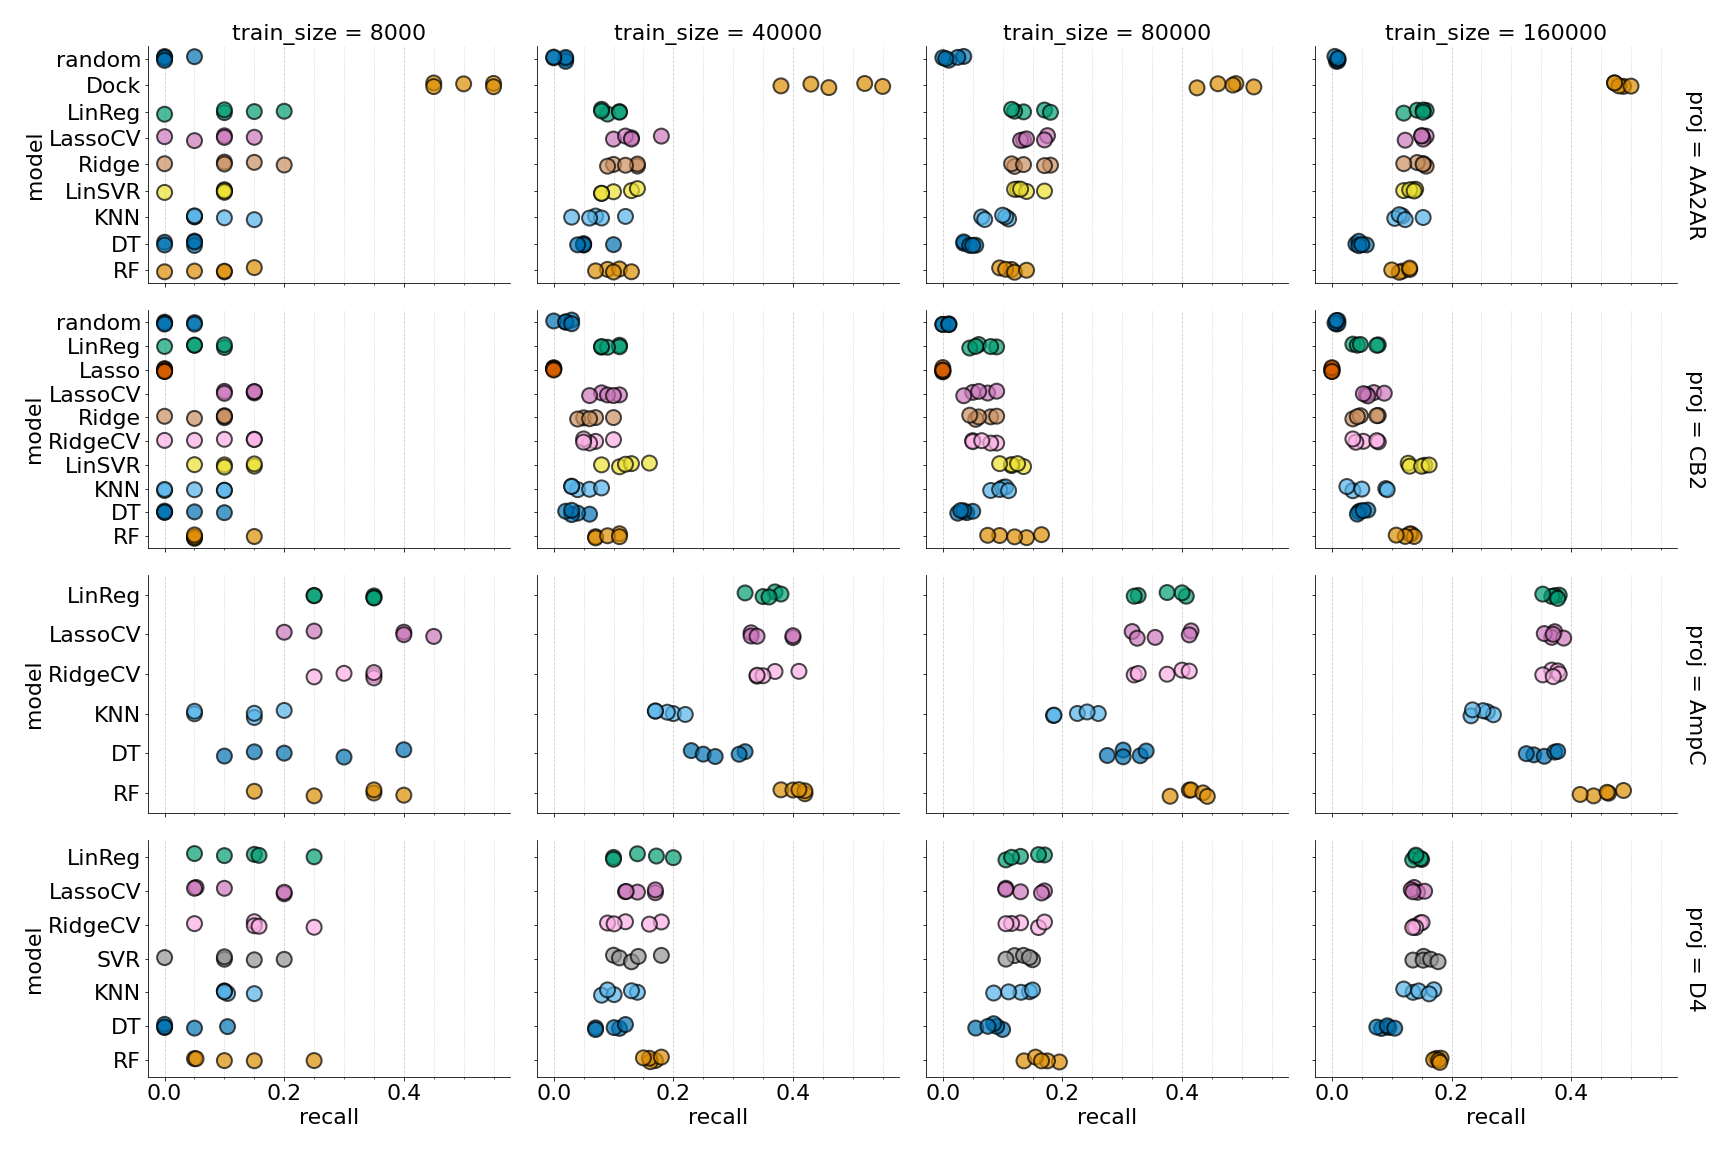
\includegraphics[width=0.8\textwidth]{figures/figure_3_single-shot-performance.png}
\caption{Model performance for multiple regression models and their baselines on 4 datasets present in the study. Rows represent different datasets, columns show different training size. Values for five independent folds are shown.}
\label{fig:fig_3_singleshot}
\end{figure}

Linear models also show more stable performance across the datasets: namely, default LinearRegression and LinearSVR show recall score similar to that of RandomForestRegressor on all datasets except for CB2, where LinearRegression shows twice smaller recall values compared to RandomForestRegressor. Interestingly, adding regularization to linear models does not increase their performance, as seen by LassoCV and RidgeCV performance.

Notably, the execution time (Figure \ref{fig:supp_fig_1_execution_time}) for the linear regression remains within few minutes, whereas more "heavyweight" algorithms take up to 100 times more for the train-predict loop even on a million-sized library, while previous works reported up to 1 day of train-predict time using modern GPUs \cite{deepdocking}.

\begin{figure}[ht]
\centering
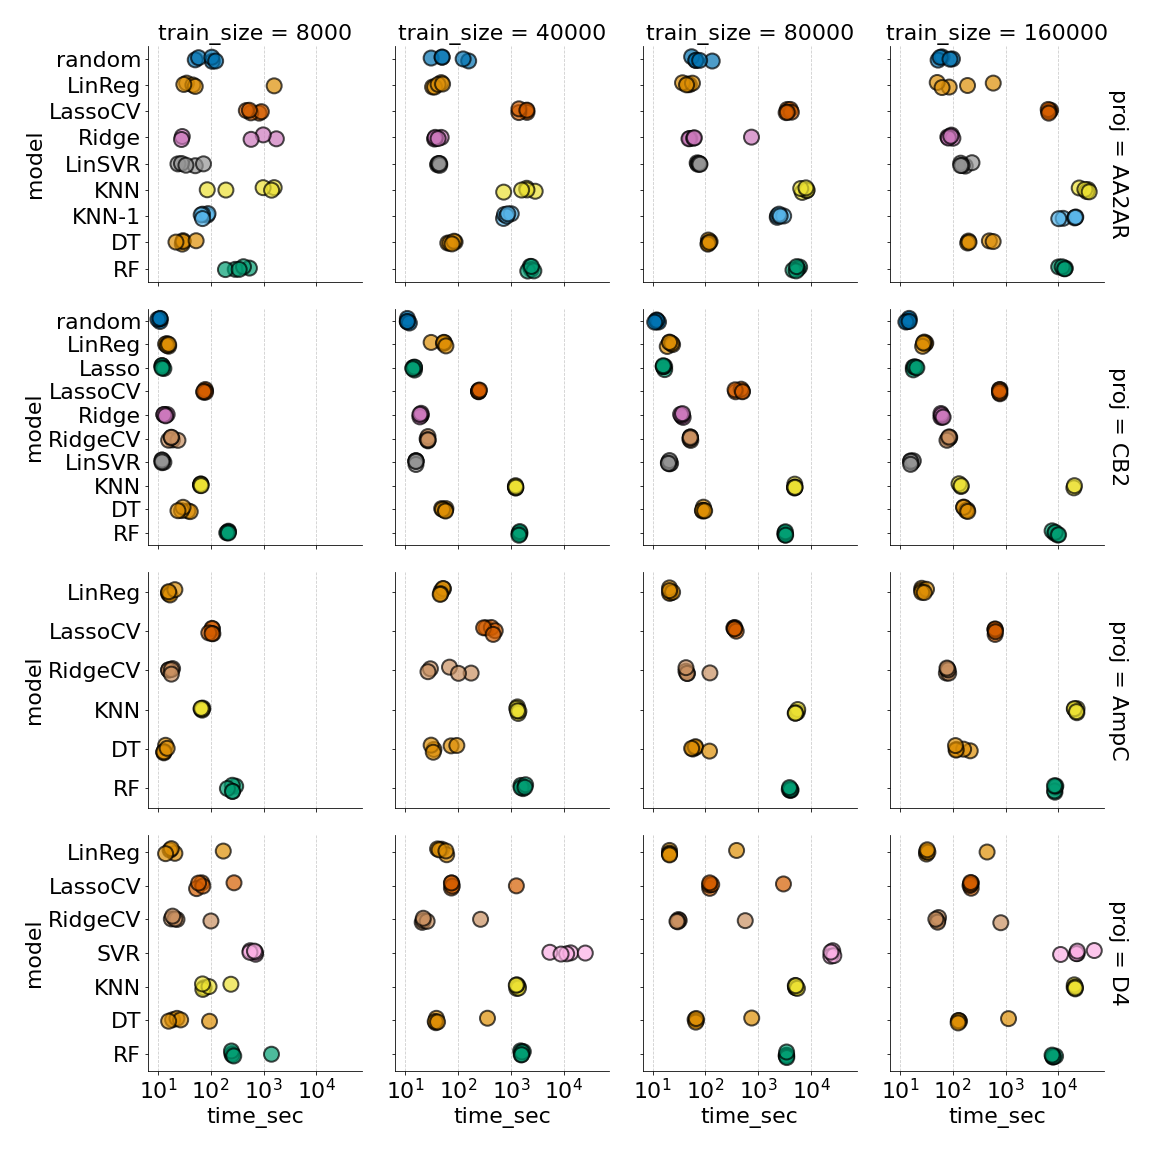
\includegraphics[width=0.8\textwidth]{figures/Supp_Figure_1_execution_time.png}
\caption{Execution time (log scale) of the train-predict loop of the algorithms evaluated in single-shot regime. Rows represent different datasets, columns -- different training size. Values for five independent folds are shown.}
\label{fig:supp_fig_1_execution_time}
\end{figure}

\subsection{Extrapolation of single-shot results}
Following the robust performance of LinearRegression in the single-shot regime, we compared the active learning regime with extrapolation from a single-shot performance, as summarized in figure \ref{fig:fig_4_extrapolation}. It is clear that for the large batch size (40 000 or 20 000), extrapolation can reliably predict an outcome of the memory-less active learning. However, with the decrease of the batch size, extrapolation seems to be overestimating the performance. Despite that, the superior performance of active learning with smaller batch size is still obvious.

\begin{figure}[ht]
\centering
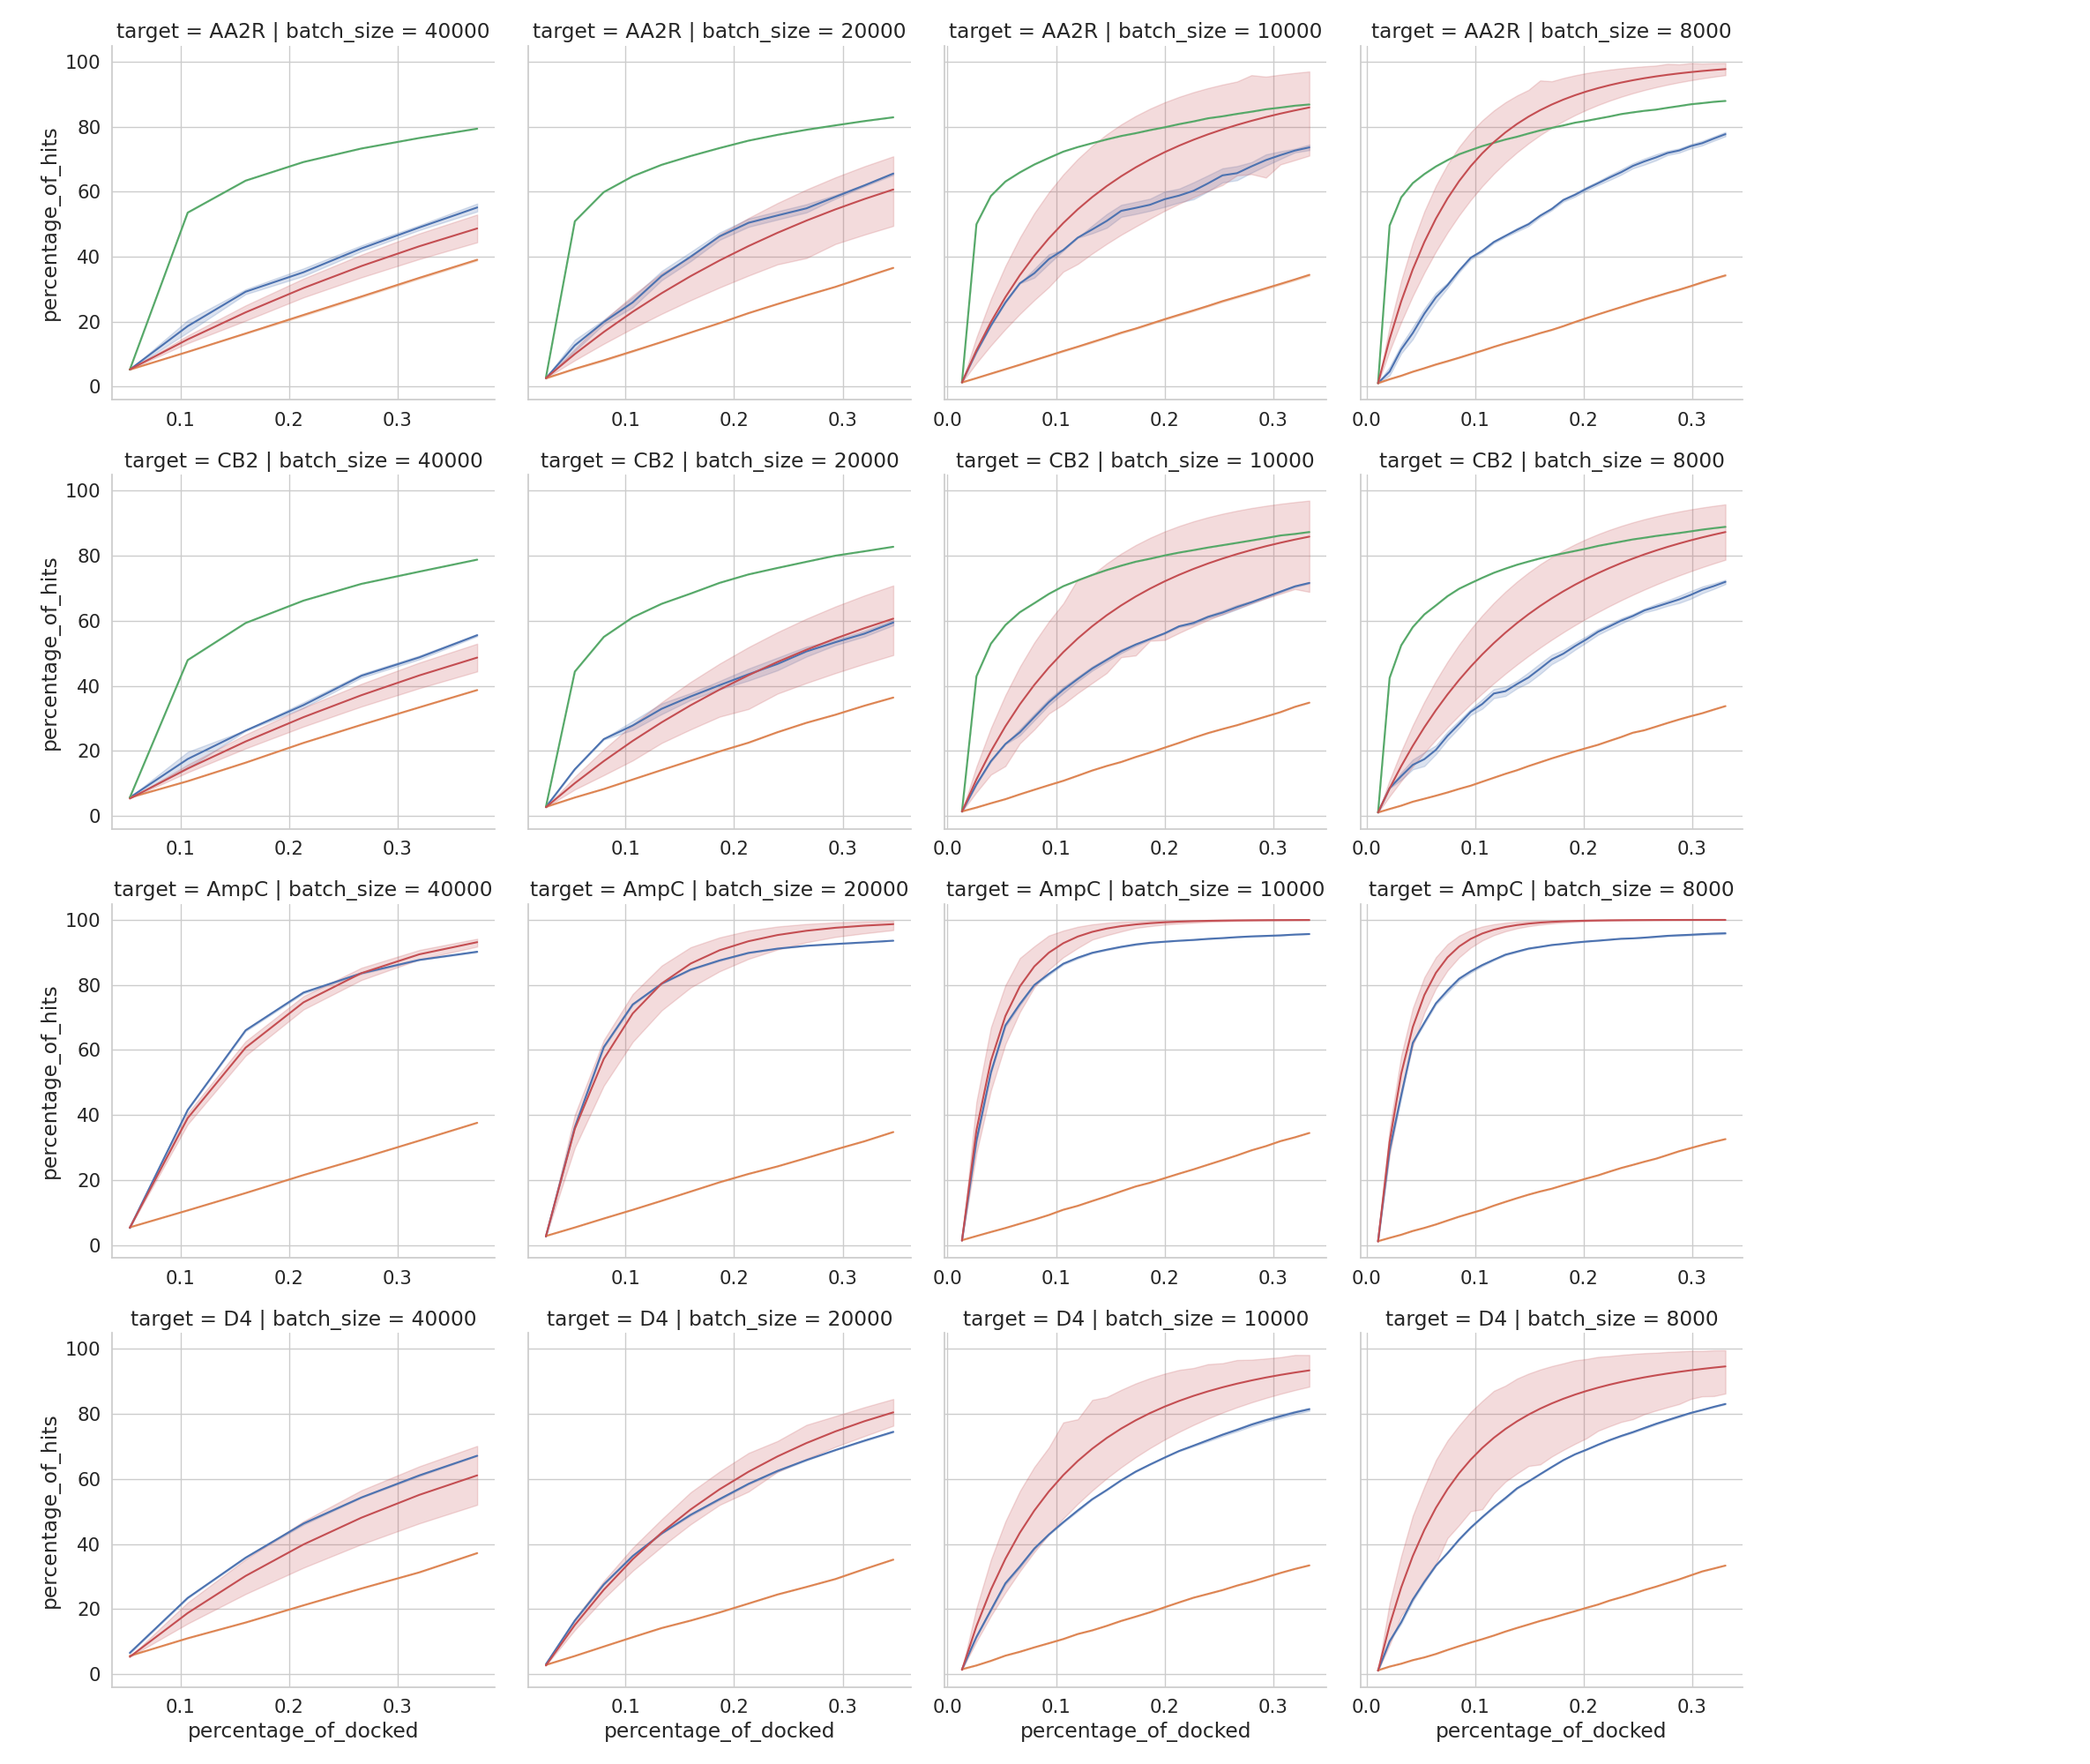
\includegraphics[width=0.8\textwidth]{figures/figure_4_iterations.png}
\caption{Comparison of the single-shot extrapolation with the simplest active learning model. Plots show cumulative percentage of hits vs percentage of the library docked, for different regimes: "LinearRegression" (actual active learning model), "RandomGaussianRegressor" (random docking score assignment baseline), "DockingAsPredictor" (using independent docking run to obtain upper-bond baseline), "Estimator" extrapolation from a single-shot performance of a LinearRegression base model.}
\label{fig:fig_4_extrapolation}
\end{figure}

It is worth noticing that results of the simple active learning model go in line with the previous results (Graff et al. \cite{Graff2021AcceleratingLearning}, as shown in figure 5): namely, after exploring six hundred thousands molecules, models with smaller batch size (0.1\%) consistently find more molecules than those with larger batch sizes (0.2\% and 0.4\%). We believe that the absolute number of docked ligands, and not the number of active learning steps, is more suitable scale for this case, since the docking itself, especially in our case of lightweight models, is the most time-consuming step.

Interestingly, when a second docking run is used as a docking score predictor, it demonstrates superior performance in the first few iterations, but then its predictions yield less real hits per step than the random search, as shown in figure \ref{fig:fig_4_extrapolation}, (datasets AA2AR and CB2). This is likely happening due to the fact that the reliably predicted VSHs are quickly exhausted at the first few steps, and the second docking is effectively useless for ligands with lower scores. Potentially, comparing success of the active learning batch prediction with the random batch prediction might serve as a stopping criteria for the real accelerated docking screening campaign.

\subsection{Optimal parameters of the active learning regime}
The meta-parameters of the active regime focused on adding memory of the docking results between different batches, as well as increasing the training size between batches. Here we discuss the \textit{early} recall (percentage of VSHs obtained after docking approx. 10\% of the library) and \textit{late} recall (after docking 30\% of the library).

As summarized in table \ref{tab:tab_1_activelearning}, models perform drastically differrent with different datasets: while for AmpC dataset, around 90\% of the VSHs are found already after screening the first 10\%, for the CB2 dataset even the best late recall is around 80\%, also requiring three times as much ligands docked. Besides, the relative model performances between different datasets are more clear.

For different meta-parameters, the decrease of the training size is also beneficial here (Table \ref{tab:tab_1_activelearning}), in agreement to the memory-less regime and the extrapolation of single-shot results. For different datasets, the smallest vs. largest batch size (40 000 vs 8 000) results in 2-3 times difference in the early recall, although difference in late recall is less significant.

Adding simple model ensembling via either MeanRank or TopFromEveryModel mechanism, or simply increasing train size (LastModel with "add" parameter) confidently boosts performance: both early and late recall is 10-15 percent points higher for all the models with a memory mechanism.

However, differences in model performance with different memory mechanisms are less obvious. If we focus on the "noadd" regime that keeps the training size constant between the batches, we can see that at batch size 8000  ensembling regime MeanRank has better performance compared to the two other methods. In this regime, each base model learns a piece of valuable information about its chemical subspace, and low-ranked molecules from a single base model still can end up in the final list of hits for the next iteration.

Interestingly, gradual increase of the train size does not boost the overall performance of the active learning regime. It increases the performance for the LastModel ensembling, effectively adding memory to the model. However, it does not increase the overall performance of other models, which already have implicit memory mechanisms. It agrees well with the single-shot performance results and the choice of simple LinearRegression models, that seem to saturate in their performance at around $16\ 000$ batch size.

Also even though the memory-less LastModel regime shows worse performance compared to others, it is still considerably higher than the performance of the random choice screening. For example, for the least performative CB2 dataset, it still finds around 34\% of the VSHs after screening only 10\% of ligands, around half of the VSHs for D4 and AA2AR datasets, and 86\% VSHs for the AmpC dataset.

\begin{table}[!ht]
    \centering
    \begin{adjustbox}{angle=90}
        \resizebox{1.2\textwidth}{!}
        {
            \begin{tabular}{|l|llllllllll|}
\hline
    \textbf{Compounds docked, \%} & \textbf{Batch size} & \textbf{Ensembling} & \textbf{Acquired hits, \%} & \textbf{} & \textbf{} & \textbf{} & \textbf{} & \textbf{} & \textbf{} & \textbf{} \\ \hline
    \textbf{} & ~ & ~ & AA2AR & ~ & CB2 & ~ & AmpC & ~ & D4 & ~ \\ 
    \textbf{} & ~ & ~ & “add” & “noadd” & “add” & “noadd” & “add” & “noadd” & “add” & “noadd” \\ 
    \textbf{10} & 40.000 & “LastModel” & 18 ± 4 & 19 ± 4 & 17 ± 5 & 17 ± 5 & 41.2 ± 0.2 & 41.6 ± 0.1 & 23.3 ± 0.5 & 23.5 ± 0.3 \\ 
    \textbf{} & ~ & “MeanRank” & 18 ± 4 & 18 ± 4 & 17 ± 5 & 17 ± 5 & 41.3 ± 0.3 & 41.2 ± 0.2 & 23.3 ± 0.5 & 23.4 ± 0.2 \\ 
    \textbf{} & ~ & “TopFromEveryModel” & 18 ± 3 & 18 ± 4 & 17 ± 5 & 17 ± 5 & 41.1 ± 0.2 & 41.2 ± 0.2 & 23 ± 1 & 23.3 ± 0.5 \\ 
    \textbf{} & ~ & Second docking & 53.8 ± 0.4 & 53.8 ± 0.2 & 47.57 ± 0.01 & 47.7 ± 0.3 & NA & NA & NA & NA \\ 
    \textbf{} & 20.000 & “LastModel” & 20 ± 8 & 26 ± 4 & 31.4 ± 0.3 & 28 ± 3 & 74.4 ± 0.4 & 74 ± 1 & 37.9 ± 0.1 & 36.35 ± 0.03 \\ 
    \textbf{} & ~ & “MeanRank” & 30 ± 7 & 28 ± 5 & 29.8 ± 0.5 & 30.5 ± 0.3 & 70 ± 1 & 72 ± 1 & 36.6 ± 0.2 & 37.8 ± 0.5 \\ 
    \textbf{} & ~ & “TopFromEveryModel” & 26 ± 8 & 25 ± 7 & 27 ± 2 & 28 ± 2 & 69.6 ± 0.4 & 70.6 ± 0.4 & 36.0 ± 0.3 & 35.6 ± 0.3 \\ 
    \textbf{} & ~ & Second docking & 64.8 ± 0.2 & 64.9 ± 0.2 & 61.1 ± 0.2 & 60.9 ± 0.3 & NA & NA & NA & NA \\ 
    \textbf{} & 10.000 & “LastModel” & 50 ± 2 & 42.1 ± 0.4 & 43 ± 3 & 39 ± 2 & 90.2 ± 0.1 & 87 ± 1 & 55.4 ± 0.3 & 46.7 ± 0.4 \\ 
    \textbf{} & ~ & “MeanRank” & 45 ± 4 & 48 ± 4 & 41 ± 1 & 44 ± 1 & 85 ± 1 & 88.6 ± 0.3 & 51.6 ± 0.4 & 54.0 ± 0.5 \\ 
    \textbf{} & ~ & “TopFromEveryModel” & 47 ± 2 & 43 ± 1 & 39 ± 6 & 36 ± 1 & 86 ± 1 & 85.3 ± 0.3 & 50.7 ± 0.3 & 47.0 ± 0.3 \\ 
    \textbf{} & ~ & Second docking & 72.25 ± 0.03 & 72.3 ± 0.1 & 70.4 ± 0.1 & 70.61 ± 0.03 & NA & NA & NA & NA \\ 
    \textbf{} & 8000 & “LastModel” & 45 ± 7 & 42 ± 1 & 40 ± 20 & 34 ± 3 & 92.4 ± 0.1 & 86 ± 1 & 61.8 ± 0.1 & 48.3 ± 0.3 \\ 
    \textbf{} & ~ & “MeanRank” & 40 ± 10 & 51 ± 3 & 39 ± 16 & 48 ± 3 & 88 ± 1 & 91.3 ± 0.4 & 56.7 ± 0.5 & 60 ± 1 \\ 
    \textbf{} & ~ & “TopFromEveryModel” & 40 ± 10 & 42 ± 3 & 40 ± 13 & 38 ± 1 & 89.2 ± 0.2 & 87.8 ± 0.3 & 56 ± 1 & 49.5 ± 0.4 \\ 
    \textbf{} & ~ & Second docking & 74.07 ± 0.02 & 74.1 ± 0.1 & 73.1 ± 0.1 & 73.2 ± 0.1 & NA & NA & NA & NA \\ 
    \textbf{30} & 40.000 & “LastModel” & 58 ± 2 & 55 ± 3 & 51 ± 4 & 56 ± 1 & 89.1 ± 0.3 & 90.2 ± 0.4 & 67.7 ± 0.3 & 67.2 ± 0.2 \\ 
    \textbf{} & ~ & “MeanRank” & 58 ± 4 & 56 ± 4 & 51 ± 5 & 53 ± 3 & 86.8 ± 0.5 & 87.8 ± 0.5 & 67 ± 1 & 68.0 ± 0.3 \\ 
    \textbf{} & ~ & “TopFromEveryModel” & 54 ± 6 & 57 ± 2 & 51 ± 7 & 53 ± 5 & 87.3 ± 0.2 & 88.4 ± 0.3 & 67± 1 & 67.1 ± 0.1 \\ 
    \textbf{} & ~ & Second docking & 79.7 ± 0.4 & 79.5 ± 0.2 & 78.5 ± 0.5 & 78.0 ± 1.0 & NA & NA & NA & NA \\ 
    \textbf{} & 20.000 & “LastModel” & 50 ± 15 & 66 ± 1 & 64 ± 2 & 60 ± 2 & 94.19 ± 0.02 & 93.6 ± 1e-14 & 76.1 ± 0.5 & 74.5 ± 0.4 \\ 
    \textbf{} & ~ & “MeanRank” & 62 ± 14 & 66 ± 3 & 63 ± 3 & 65 ± 3 & 92.3 ± 0.3 & 93.2 ± 0.4 & 74.8 ± 0.2 & 75.6 ± 0.4 \\ 
    \textbf{} & ~ & “TopFromEveryModel” & 63 ± 5 & 65 ± 3 & 63 ± 2 & 63 ± 2 & 93.1 ± 0.3 & 94.3 ± 0.2 & 74.6 ± 0.1 & 74.4 ± 0.4 \\ 
    \textbf{} & ~ & Second docking & 82.9 ± 0.2 & 82.7 ± 0.2 & 83.0 ± 0.1 & 82.9 ± 0.2 & NA & NA & NA & NA \\ 
    \textbf{} & 10.000 & “LastModel” & 79 ± 2 & 74 ± 2 & 73 ± 2 & 71.6 ± 0.4 & 97.0 ± 0.1 & 95.6 ± 0.1 & 85.6 ± 0.3 & 81 ± 1 \\ 
    \textbf{} & ~ & “MeanRank” & 70 ± 10 & 82 ± 1 & 73 ± 4 & 76.8 ± 0.2 & 96.2 ± 0.4 & 96.2 ± 0.2 & 84.3 ± 0.1 & 84.8 ± 0.2 \\ 
    \textbf{} & ~ & “TopFromEveryModel” & 78 ± 7 & 78 ± 1 & 68 ± 10 & 72 ± 1 & 96.8 ± 0.1 & 97.0 ± 0.1 & 84.1 ± 0.1 & 81.8 ± 0.2 \\ 
    \textbf{} & ~ & Second docking & 86.68 ± 0.01 & 86.80 ± 0.02 & 87.3 ± 0.1 & 87.5 ± 0.2 & NA & NA & NA & NA \\ 
    \textbf{} & 8000 & “LastModel” & 76 ± 10 & 78 ± 2 & 70 ± 20 & 72 ± 2 & 97.5 ± 0.1 & 96 ± 1 & 88.1 ± 0.4 & 83.1 ± 0.3 \\ 
    \textbf{} & ~ & “MeanRank” & 75 ± 6 & 85 ± 1 & 70 ± 20 & 80.3 ± 0.4 & 96.9 ± 0.1 & 96.8 ± 0.1 & 86.7 ± 0.1 & 87.6 ± 0.3 \\ 
    \textbf{} & ~ & “TopFromEveryModel” & 77 ± 5 & 80 ± 2 & 69 ± 15 & 75 ± 1 & 97.3 ± 0.1 & 97.5 ± 0.1 & 86.9 ± 0.2 & 84.0 ± 0.1 \\ 
    \textbf{} & ~ & Second docking & 88.1 ± 0.1 & 88.0 ± 0.1 & 88.8 ± 0.3 & 88.89 ± 0.01 & NA & NA & NA & NA \\ \hline
\end{tabular}

        }
    \end{adjustbox}
    \caption{Figure 5: Recall score of the early stage (after 10\% library screened) and late stage (after 30\% library screened). Errors represent standard deviation within five independent folds.}
    \label{tab:tab_1_activelearning}
\end{table}